\documentclass{article}
\usepackage[utf8]{inputenc} 
\usepackage[spanish,es-tabla,es-nodecimaldot]{babel}
\usepackage{graphicx}
\usepackage{amsmath}
\usepackage{csvsimple}
\usepackage{authblk}
\usepackage{cprotect}
\usepackage{floatrow}
\usepackage[caption=false]{subfig}
\usepackage{booktabs}
\usepackage{hyperref}
\usepackage{lscape}
\usepackage{gensymb}
\usepackage[a4paper,top=3cm,bottom=2cm,left=3cm,right=3cm,marginparwidth=1.75cm]{geometry}
\usepackage{siunitx}
\usepackage[square,sort,comma,numbers]{natbib}
\usepackage[nottoc,numbib]{tocbibind}
\usepackage{float}
\usepackage{pgfplotstable}
\floatstyle{plaintop}
\restylefloat{table}



\author{Nepo Rojas}

\title{Introducción a la Programación en R para Análisis de Datos Físicos \\ \begin{large}
    Actividad 1: Cálculo de variables y resumen de los datos \end{large}}

\begin{document}

\maketitle

El código con el que generamos los resultados de este reporte lo encontrarás
\href{https://github.com/niesfutbol/sport_scientists/blob/develop/src/activity_1.R}{sport\_scientists/src/activity\_1.R}.
El código podría diferir del presente en este reporte. La versión actualizada del código está en la
liga al repositorio.

En la figura \ref{fig:genralStructure} vemos la estuctura general de la base de datos. La base de 
datos tiene 23 renglones y 23 columnas. En el recuadro rojo vertical podemos ver los tipos de
variables. Las primeras cuatro columnas son cadenas de caracteres y el resto son números.
\begin{figure}[H]
    \centering
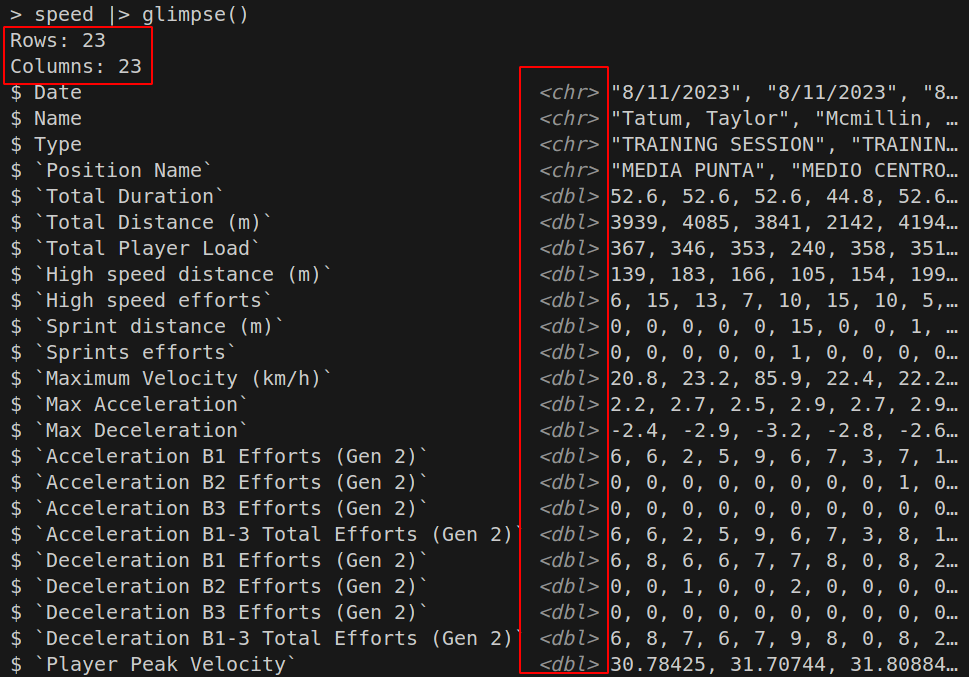
\includegraphics[scale=0.6]{../static/activity_1_2.png}
\caption{Captura de pantalla con la estructura general de la bases de datos. Información obtenida a 
partir de la función \texttt{glimpse()}.}
\label{fig:genralStructure}
\end{figure}

Al explorar los datos notamos que el jugador \textbf{Grant, Joshua} no tiene datos, su duración es
0. Así que lo retiramos de la base de datos:
\begin{verbatim}
player_without_info <- speed |>
  filter(total_duration == 0) |>
  pull(name)

cleaned_speed <- speed |>
  filter(total_duration != 0)
\end{verbatim}


\subsubsection*{Distancia total acumulada por posición}
En la figura \ref{fig:meanSpeedPosition} vemos distancia total acumulada por encima de 21km/h
promedio por cada posición. Los registros están acomodados de menor a mayor.
\textbf{Media punta} es la posición con menor distancia acumulada y con la mayor distancia
acumulada promedio fue \textbf{Medio centro}.
\begin{figure}[H]
\centering
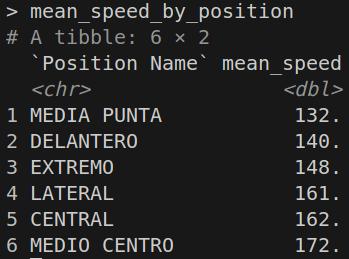
\includegraphics[scale=0.6]{../static/activity_1_5.png}
\caption{Captura de pantalla con la rapidez promedio por posición. La información la obtuvimos a 
partir de la función \texttt{summarize()}.}
\label{fig:meanSpeedPosition}
\end{figure}

\subsubsection*{Velocidad máxima de los jugadores}
Revisamos el máximo en la velocidad de los jugadores:
\begin{verbatim}
max_speed <- cleaned_speed |>
  pull(`Maximum Velocity (km/h)`) |>
  max()
\end{verbatim}
El valor que encontramos fue de 85.9 km/h. De la
\href{https://es.wikipedia.org/wiki/100_metros}{Wiki} sabemos que el record mundial lo tiene Usain
Bolt con una rapidez de 42 km/h. Asi que tiramos todos los registros por arriba de 40 km/h:
\begin{verbatim}
cleaned_speed <- cleaned_speed |>
  filter(`Maximum Velocity (km/h)` < 40)
\end{verbatim}


\subsubsection*{Rapidez promedio, porcentaje de velocidad máxima y aceleraciones de alta intensidad}
Calculamos la rapidez promedio de cada jugador como la división de la distancia que recorrió en la
sesión entre la duración de la sesión. También buscamos el porcentaje de la velocidad máxima
registrada para cada jugador. Es decir, comparamos la valocidad máxima de referencia de cada jugador
contra la máxima alcanzada en esta sesión. Por último calculamos, el número de aceleraciones de alta
intensidad, es decir el número de aceleraciones que fueron mayores a 2 m/$s^2$:
\begin{verbatim}
new_speed <- cleaned_speed |>
  mutate(
    mean_speed = total_distance / total_duration,
    percentage_max_speed = `Maximum Velocity (km/h)`*100/`Player Peak Velocity`,
    high_intensity_acceleration = `Acceleration B2 Efforts (Gen 2)` + `Acceleration B3 Efforts (Gen 2)`
  )
\end{verbatim}
La figura \ref{fig:numericSummary} es una captura de pantalla del resumen numérico de las variables
que calculamos arriba. Vale la pena notar que las unidades de la velocidad promedio es m/min. Así la
rapidez promedio máxima de 91.5 m/min es equivalente a 5.49 km/h.
\begin{figure}[H]
\centering
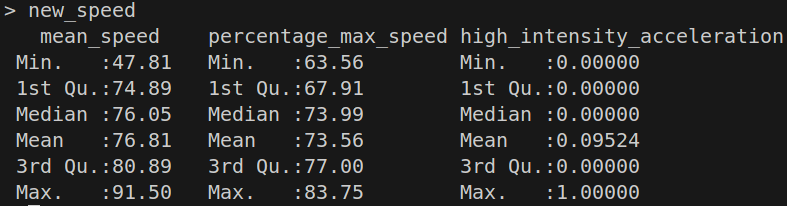
\includegraphics[scale=0.6]{../static/activity_1_8.png}
\caption{Captura de pantalla con el resumen numérico de las variables rapidez promedio (m/min),
porcentaje de velocidad máxima y (número de) aceleraciones de alta intensidad. La información la
obtuvimos a partir de la función \texttt{summary()}.}
\label{fig:numericSummary}
\end{figure}
\end{document}
